% TODO: Add n.d. as year entry for bib entries that don't have a date. (Search for "()" in the PDF)
% TODO: Fix page breaks before captions

\documentclass{article}
\usepackage[hidelinks]{hyperref}
\usepackage{csquotes}
\usepackage[vmargin=25mm, hmargin=20mm]{geometry}
\usepackage{xcolor}
\usepackage{graphicx}
\usepackage{float}
\usepackage{pgfplots}
\usepgfplotslibrary{colorbrewer}
\pgfplotsset{compat = 1.18} 
\usetikzlibrary{pgfplots.statistics, pgfplots.colorbrewer} 
\usepackage{pgfplotstable}
\usepackage{listings}
\lstset{
    backgroundcolor=\color[RGB]{240, 240, 240},   
    basicstyle=\ttfamily\footnotesize,
    breakatwhitespace=false,
    breaklines=true,
    keepspaces=true,
    numbers=left,
    numbersep=5pt,
    showspaces=false,
    showstringspaces=false,
    showtabs=false,
    tabsize=4,
    postbreak=\mbox{\textcolor{red}{$\hookrightarrow$}\space},
    aboveskip=10pt
}
\usepackage[
    backend=biber,
    sorting=none,
    style=ieee,
    urldate=long,
    maxcitenames=2,
    mincitenames=1
]{biblatex}
\addbibresource{sources.bib}
\usepackage{multicol}
\setlength{\columnsep}{13mm}
\usepackage{hypcap}
\usepackage{caption}
\captionsetup{
    justification=centerlast,
    font=small,
    labelfont=sc,
    margin=5pt,
    belowskip=15pt
}
\DeclareCaptionType{listing}[Listing][List of Listings]

\title{%
\vspace{50px}%
    \Huge Differential Fuzzing on coreutils Using LibAFL\break%
    —\break%
    Report%
    \vspace{250px}%
}

\author{%
  Valentin Huber\vspace{5px}\\%
  \small \href{https://www.zhaw.ch/en/engineering/institutes-centres/init/}{Institute of Applied Information Technology}\\%
  \small \href{https://www.zhaw.ch/en}{Zürich University of Applied Sciences ZHAW}\\%
  \small \href{mailto://contact@valentinhuber.me}{contact@valentinhuber.me}%
  \vspace{10px}
}
\date{\today\vspace{5px}}

\DeclareFieldFormat*{citetitle}{\textit{#1}}
\hfuzz=50px
\hbadness=10000
\newcommand{\code}[2][]{\lstinline[language=#1, breaklines=false, basicstyle=\ttfamily\normalsize]{#2}}
\let\savedCite=\cite
\renewcommand{\cite}{\unskip~\savedCite}
\let\savedRef=\ref
\renewcommand{\ref}{\unskip~\savedRef}

\begin{document}
\pagenumbering{gobble}
\maketitle

\clearpage\newpage
\begin{center}
    \begin{minipage}{0.8\textwidth}
        \vspace{70px}
        \begin{abstract}
            Hello, %
            %
            World!
        \end{abstract}
    \end{minipage}
\end{center}

\clearpage\newpage
\newgeometry{vmargin=25mm, hmargin=40mm}
\tableofcontents
\clearpage\newpage
\restoregeometry
\pagenumbering{arabic}

\begin{multicols}{2}
    \section{Introduction}

    Fuzz testing has developed into an important tool for finding software defects. By repeatedly running a program under test with varied input data and detecting illegal states such as crashes, it is an automated alternative to manual security and reliability testing. Introduced in \citeyear{UNIX} in the seminal work by \citeauthor{UNIX}\cite{UNIX}, it is now widely used in industry. Companies such as Google, Microsoft, Cisco, or Adobe and governmental agencies such as the US Department of Defense have developed proprietary fuzzers or contributed to open source fuzzers. Fuzz testing has proven an effective tool for both security and reliability testing. Its accolades include, among others, 20,000 discovered vulnerabilities in Google's Chrome browser alone.\cite{Demystifying}

    \subsection{Differential Fuzzing}
    \label{IntroductionDifferentialFuzzing}

    While extensive research has been conducting on fuzzing, one field which has not received a lot of attention is the oracle which defines what an illegal state of the program under test constitutes. While simple oracles such as program crashes and timeouts are easy to detect, further exploration has not gone past very general logic, such as memory-violation bugs.\cite{SurveyRoadmap}

    One such oracle is what is used in so-called differential fuzzing. It relies on two independent implementations of the same underlying program logic and works by comparing their output under the same input. Compared to other common and more general oracles, this allows detecting logic errors that do not invalidate basic guardrails such as memory access rules.

    \subsection{coreutils}

    This work will examine coreutils as an example of a target to perform differential fuzzing on. coreutils are a suite of programs that allow users to interact with their system on the command line. Popularized by the version developed by the GNU project and available on almost all current Linux systems, utilities such as \code{ls}, \code{cat}, \code{base64}, \code{grep}, \code{env}, or \code{whoami} are indispensible tools for many users' daily workflows. Section~\ref{Coreutils} will provide a more in-depth introduction to coreutils along with information about its history, interface and technical build-up.

    \subsection{LibAFL}
    \label{LibAFLHistory}

    American Fuzzy Lop (AFL)\cite{AFL} was one early comprehensive open-source fuzzing tool used in countless projects and academic works to detect an impressive list of software defects and security vulnerabilities\cite{AFLBugs}. After it was no longer updated in November 2017, the fork AFL++\cite{AFLPlusPlus} has become the de facto replacement.

    However, while advancements on AFL++ have been introduced in many academic and commercial projects, because of the architecture of AFL++, these usually have not been introduced back to AFL++. This results in a list of incompatible forks, each with a proven improvement that makes the fuzzer more effective at its job.\cite{LibAFL} Because of this, the maintainers of AFL++ started a new project: LibAFL. It aims to provide a toolkit for building fuzzers that is flexible enough to allow combination of all these advancements. Refer to Section~\ref{LibAFLBackground} for more details on LibAFL. This work uses LibAFL to build a fuzzer aimed to find software defects in coreutils.

    \subsection{Research Questions}
    \label{ResearchQuestions}

    The remainder of this work aims to answer the following questions:

    \begin{enumerate}
        \item Which parts of coreutils can be fuzzed? What performance tradeoffs does each part introduce?
        \item How can the necessary instrumentation be introduced into coreutils? What are the engineering and performance implications of each option?
        \item Can LibAFL feasibly be used to build a system with all logic defined in the answers to the questions above?
        \item If yes, how effective is the resulting fuzzer at finding bugs in coreutils? What kind of bug can be found with it?
        \item Can the system be expanded to implement differential fuzzing between the different implementations? What changes are necessary?
        \item If yes, how effective is the this second fuzzer at finding bugs in coreutils? What kind of bug can be found with it?
    \end{enumerate}

    Refer to Section~\ref{ResearchQuestionsDiscussion} for a summary of the answers produced in this work.

    \section{Background}

    To understand the requirements to and the architecture of the fuzzer, some background information on coreutils and LibAFL's architecture are necessary. This section provides an overview of these topics.

    \subsection{coreutils}
    \label{Coreutils}

    On \citedate{FileUtilsAnnouncement}, {\DeclareNameAlias{labelname}{given-family}\citeauthor{FileUtilsAnnouncement}} announced fileutils, a suite of utilities for reading and altering files\cite{FileUtilsAnnouncement}. A year later, he released textutils (to parse and manipulate text)\cite{TextUtilsAnnouncement} and shellutils (to write powerful shell scripts)\cite{ShellUtilsAnnouncement}. These three collections were folded into one on \citedate{CoreUtilsAnnouncement}, called the GNU coreutils.\cite{CoreUtilsAnnouncement} \code{ls}, \code{cat}, \code{base64}, \code{grep}, \code{env}, or \code{whoami}: GNU's coreutils are at the basis of how users interact with most Linux distributions on the command line.\cite{GNULinux} Because they are so widely used and central to how users interact with their computers, software quality and lack of software defects is especially important to coreutils.

    Version 9.5 of the GNU coreutils was released on \citedate{GNUCoreUtils9.5} and thus marks the current version as of this report. 106 programs are built per default.\cite{GNUCoreUtils9.5}

    \subsubsection{Interface}
    \label{CoreutilsInterface}

    Users primarily interact with coreutils through the command line or in shell scripts. They take different kinds of inputs, i.e. behave differently based on changes to:
    \begin{itemize}
        \item Data passed to \code{stdin}, e.g. through Unix pipes
        \item Command line arguments:
              \begin{itemize}
                  \item Unnamed arguments, either required (such as \code{cp <source> <destination>}) or optional (such as \code{ls [directory]})
                  \item Flags without any associated data, such as \code{--help}
                  \item Flags with associated data, either required (such as \code{dd} \code{if=<input file>} \code{of=<output file>}) or optional {such as \code{-name <pattern>} in \code{find}}
              \end{itemize}
        \item Environment variables, such as \code{LANG}
        \item The file system content, such as for \code{ls}
    \end{itemize}

    The output, or effects of invocations fall into the following categories:
    \begin{itemize}
        \item Data written to \code{stdout}
        \item Data written to \code{stderr}
        \item The exit status of the process
        \item The signal terminating the process
        \item Changes to the file system
    \end{itemize}

    \subsubsection{Alternative Implementations}

    Since the release of GNU coreutils, multiple alternative implementations were released. Notable among those are BusyBox\cite{BusyBox}, which aims to provide most of the GNU coreutils with a focus on resource restrictions. It is therefore primarily used in embedded systems\cite{BusyBox} or tiny distributions such as Alpine Linux\cite{Alpine}.

    In the general push towards rewriting software in memory-safe languages, the uutils project\cite{Uutils} maintains a drop-in replacement implementation of the GNU coreutils written in Rust.\cite{UutilsCoreUtils} It does contain all programs, but is still missing certain options. All differences with GNU's coreutils are treated as bugs. It further aims to not only work on Linux, but is also available for MacOS and Windows.

    \subsubsection{Build System}
    \label{CoreutilsBuildSystem}

    The GNU coreutils employ a complex, multi-step build system, including Autoconf\cite{Autoconf} and Automake\cite{Automake}. Changes to either the code or the build system configuration require a deep understanding of the entire ecosystem to ensure no unintended changes to the resulting binaries are introduced. uutils' version of coreutils relies on cargo as its build system, which make outcomes of changes to the code much more predictable.

    \subsection{LibAFL}
    \label{LibAFLBackground}
    As introduced in Section~\ref{LibAFLHistory}, LibAFL is an extendible framework to build custom fuzzers. What follows is a short introduction to the ideas and parts of LibAFL necessary to understand this project. For a more in-depth look, the authors refer to the original LibAFL paper\cite{LibAFL}.

    \subsubsection{Generic Concepts}
    The core insight by the authors of LibAFL is that most fuzzers contain very similar parts, where advancements in new works are usually developments in only few of the fundamental fuzzer parts. The logic is usually either introduced into a fork of an existing fuzzer (such as AFL++), which is then abandoned without collecting the advancements in a way that they are reusable and combinable in later projects. Alternatively, authors might elect to create a new system from scratch, which introduces a lot of duplicate work and code, which isn't as optimized as possible, since fuzzer parts such as the thread synchronization usually aren't the focus of new works.

\end{multicols}
\begin{figure}[htbp]
    \centering
    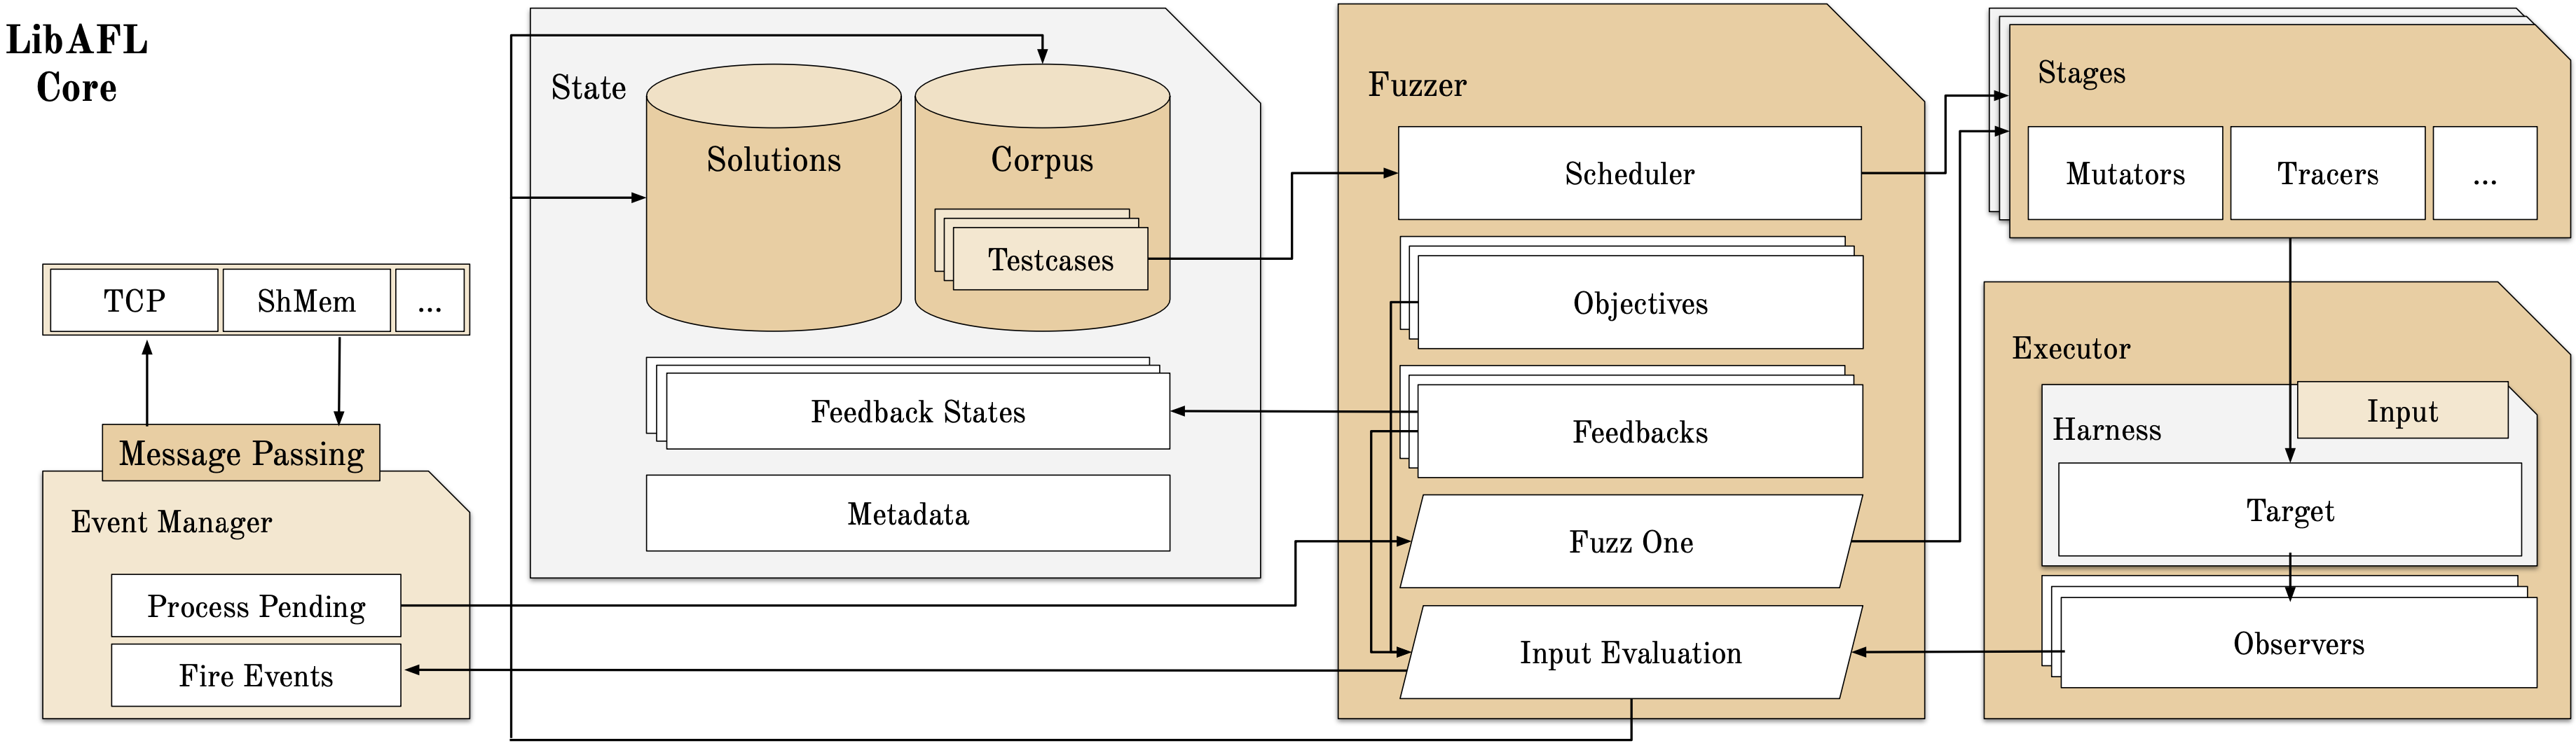
\includegraphics[width=\textwidth]{assets/LibAFLArchitecture.png}
    \caption{LibAFL's Architecture\cite{LibAFL}}
    \label{fig:LibAFLArchitecture}
\end{figure}
\begin{multicols}{2}

    The authors of LibAFL examined recent innovations in fuzzing and identified a set of distinct parts present in many of the fuzzers. They then designed the architecture of LibAFL in such a way that authors can change just the parts they are interested in and rely on a well-optimized default implementation for everything else. Figure\ref{fig:LibAFLArchitecture} shows the identified fuzzer parts and their interaction, as implemented in LibAFL. Using this architecture, the authors of LibAFL re-implemented the logic introduced in high-impact 20 works to both proof that the system is flexible enough to handle logic created indepen from their system. Finally, they showed that it is now trivial to combine advancements made in different works (i.e. combining the input scheduler of one work with new feedback types introduced in another).

    \subsubsection{Usage of Traits}
    \label{LibAFLTraits}

    On a more technical side, to achieve their goal, the authors heavily relied on Rust's trait system in combination with generic types. This section will present a selection of these core traits, including a short explanation. For a complete list and more expansive documentation, the author refers to the paper which introduced LibAFL\cite{LibAFL} and the official LibAFL book\cite{LibAFLBook}.

    \paragraph{Executor}

    The \code{Executor} is called with a certain \code{Input} and executes the program under test. It ensures that the passed \code{Observer}s can gather whatever information they need to and provide additional information about the execution run. Examples for \code{Executors} include \code{InProcessExecutor}, which calls the provided function directly, \code{InProcessForkExecutor}, which calls \code{fork} before calling the function and trades off additional performance overhead for improved stability. Finally, while being libraries external to the LibAFL core, \code{FridaInProcessExecutor} and \code{QemuExecutor} use the dynamic instrumentation framework Frida resp. the emulator QEMU to support complex fuzzing approaches.

    \paragraph{Observer}

    \code{Observer}s are passed to an \code{Executor} and gather information before, during, or after the execution. This information can take any arbitrary shape. Typical \code{Observer} implementations used in fuzzers include \code{StdMapObserver}, which is often used to keep track of coverage data by recording execution paths, or \code{CmpObserver} to trace comparisons during an execution run.

    \paragraph{Feedback}

    There are two uses for \code{Feedback}s in LibAFL: objectives and feedbacks steering the search. They reduce a combination of information provided by the \code{Executor} and \code{Observer}s to a boolean value: Is this test case interesting? If used as an objective, this marks the test case in question as a solution. If used as a steering feedback, it will add the current test case to the corpus from which (after mutating it) the next input is drawn. Typical examples include a \code{CrashFeedback}, \code{TimeoutFeedback} (both usually used in the objective mode) and a \code{MaxMapFeedback}, which can be used to see if new parts of the memory map used to keep track of the executed parts of the binary are touched, thus representing the coverage-guided part of the fuzzer.

    \paragraph{Input}

    \code{Input}s are about what one would expect: A representation of what is mutated and then passed to the \code{Executor}. Typically, it consists of a simple variable length byte array, but may also be a more complex \code{struct}. Depending on the use case, the former might be sufficient or one might need the additional flexibility provided by the latter.

    \paragraph{Mutator}

    Finally, \code{Mutator}s take an \code{Input} and change it in some form. On simple byte array \code{Input}s, this may be flipping a bit, or injecting an additional byte somewhere. For more complex \code{Input}s, custom \code{Mutator}s may need to be written. All \code{Mutator}s included in a certain fuzzer are passed to a scheduler which mutates an \code{Input} once or multiple times with the received \code{Mutator}s. This is another example of the flexibility of LibAFL: While one may need to write custom \code{Mutator}s for a custom \code{Input} type, all scheduling algorithms available in LibAFL can be used regardless, without any additional changes.

    \section{Implementation}
    \label{Implementation}

    This section introduces the concepts and technical details necessary to reproduce the findings of this work by incrementally adding capabilities to a fuzzer. The example fuzzer will target \code{base64}, a comparatively small program from the coreutils. It encodes and decodes binary data to a format consisting only of characters unproblematic in most contexts. It takes its input from either a file or \code{stdin} and provides the following options:
    \begin{itemize}
        \item \code{--decode} switches \code{base64}'s mode from encode to decode
        \item \code{--ignore-garbage} ignores non-alphabet characters when decoding
        \item \code{--wrap <cols>} inserts linebreak after \code{<cols>} characters when encoding
        \item \code{--help} prints information about \code{base64} and exits
        \item \code{--version} prints version information and exits
    \end{itemize}

    \subsection{Basic Unguided Fuzzer}

    The first step is to build a fuzzer without any features: It just takes a byte array, randomly mutates it, feeds it to the fuzzer and checks for crashes. It does not contain any execution steering nor can it trigger the different options. One can choose the default implementations for each part outlined in Section\ref{LibAFLBackground}, which reduces the necessary code for the fuzzer to well under 100 lines. However, this fuzzer is very unlikely to find any software defect, since it essentially employs the same strategy as was proposed in the seminal work by \citeauthor{UNIX} in \citeyear{UNIX}: inserting random data into a program and hoping for a crash, without any additional logic. Additionally, it does not even have access to all parts of the program, since the command line arguments are never used.

    \subsubsection{Environment Protection}
    \label{Environment}

    The most simple solution to allow a fuzzer to access the command line arguments would be to split the byte array at a magic byte (e.g. \code{NULL} bytes), and pass the first entry to \code{stdin} and all remaining as command line arguments. However, this introduces a problem: Some programs in the coreutils can change the environment they are running in, as described in Section~\ref{CoreutilsInterface}. This may be entirely trivial (e.g. creating and writing to a temporary file in an unrelated part of the filesystem), but may also disturb the fuzzing process or even incur irreparable damage to the system by overwriting critical files.

    The fuzzer therefore needs to protect the environment from the effects of the program. This can be done in a few different ways, each of which introduces a certain downside:
    \begin{enumerate}
        \item First, the fuzzer could create a layered filesystem and use it to create an environment for the program under test to run in. This is what Docker uses to use the host's kernel while fooling the program under test into thinking it runs natively. Changes to the file system are captured and stored while read operations are responded to with data from the write layer if it has been changed previously and from the host's file system if not. However, the performance implications of this approach are immense: While starting a coreutils program takes about 20~ms on the author's system, starting a Docker container takes approximately 2~s. Additionally, doing this across many cores, as is typical in modern fuzzing, relies on the parallelization of starting containers as done by the Docker daemon. This is not necessarily the case, in fact in earlier work by the author\cite{VT1}, sub-linear scaling effects could be observed.
        \item Alternatively, a dynamic translation layer could be introduced that captures the relevant syscalls and handles them appropriately. While this would limit the startup overhead, it would slow down the program execution. Additionally, the logic necessary in the dynamic environment protection layer is non-trivial and may depend on both the program under test and the specific system used to run the fuzzer.
        \item Many programs in the coreutils don't change the environment they run in, or only do so for very specific options. So while unable to reach all code, restricting the fuzzing campaigns to the program parts which do not change their environment would prevent any performance overhead at the cost of completeness. This is the approach pursued in this project.
    \end{enumerate}

    \subsubsection{Custom Input Type}
    \label{CustomInputType}

    This approach requires restricting the fuzzer to only execute whitelisted parts of the program under test, specifically to only add certain command line arguments. This also means that certain parts of the command line argument parsing routines will never get tested, since only valid command line arguments will be tested. The associated data to a certain flag (see Section~\ref{CoreutilsInterface}) may still be invalid and the corresponding parsing routine will be tested.

    Since this project uses LibAFL, this can be achieved quite easily by implementing a custom \code{Input} type (refer to Section~\ref{LibAFLTraits}). By introducing a trait which contains functions that map the \code{Input} to the arguments necessary for the \code{Executor}, it is possible to build a system where the only addition to the codebase for additional programs to test is adding
    \begin{itemize}
        \item a custom \code{Input} struct,
        \item a mapping function for the \code{Executor},
        \item a few simple trait implementations needed for the fuzzer (such as \code{Display}), with many necessary implementations available as \code{derive}s,
        \item a \code{Generator} for the above, which will generate random seeds for the fuzzer to start from, and
        \item a set of \code{Mutator}s, which will mutate the parts of the \code{Input} independently. For this part, the author introduced a system which allows reusing the default byte array mutators for any \code{Input} part consisting of a byte array.
    \end{itemize}

    \subsection{Optimizations}
    \label{Optimizations}

    This basic fuzzer can then be augmented by systems that LibAFL provide. With very little additional code, the fuzzer can be extended to run on all available cores or even multiple machines, use advanced algorithms to choose the best \code{Mutator}, etc. Additional \code{Observer}s and \code{Feedback}s, such as a \code{TimeoutFeedback} can be introduced with no additional configuration. This is where LibAFL as a framework simplifies building an advanced fuzzer significantly.

    \subsection{Gathering Coverage Information from GNU coreutils}
    \label{CoverageGNU}

    To test any non surface level code, the fuzzer needs information of some form about what parts of the binary just got executed. This coverage information can fundamentally be gathered in two ways: Either the necessary logic is compiled into the binary, or it is added dynamically. While the former is more performant, it also requires changes to the binary. And as described in Section~\ref{CoreutilsBuildSystem}, making changes to the code or build system of GNU coreutils is a complex task. Previous experiments by the author on coreutils showed that in principle, adding compile-time coverage-gathering instrumentation is possible.\cite{VT1}

    \subsubsection{LibAFL's Coverage Interface}
    \label{LibAFLCoverageInterface}

    LibAFL heavily relies on shared memory maps for a wide range of internal functionality like corpus synchronization across threads. It is further important for different kinds of \code{Feedback}, especially coverage information. Its built-in logic for adding coverage gathering instrumentation to a binary to test relies on passes in the clang compiler, specifically the \code{SanitizerCoverage}\cite{SanitizerCoverage} module. This module includes different levels of coverage instrumentation, the examples provided by LibAFL typically use \code{trace-pc-guard}. This will insert the call shown in Listing~\ref{listing:EdgeFunction} on every edge.

    \begin{lstlisting}[language=C]
__sanitizer_cov_trace_pc_guard(&guard_variable)
\end{lstlisting}
    \captionof{listing}{Inserted Call on Every Edge}
    \label{listing:EdgeFunction}

    The implementation of this function is then left for the developer.  The LibAFL module \code{libafl\_targets} provides such implementations which allocate a shared memory map with the correct size and then on the execution of each edge marks the memory section associated with it. Finally, a \code{MaxMapFeedback} is used as feedback in the fuzzer, which makes the fuzzer prioritize inputs that visited new paths in the binary under test, since additional bits are set in the shared memory map.

    However, these default implementations only work if the fuzzer and binary under test exist in the same process, i.e. when the fuzzer and source code to test are compiled into a single unit. Based on the reasoning in Section~\ref{CoreutilsBuildSystem}, this is not a feasible solution for this project. Hence, a different approach was created.

    \subsubsection{Instrumentation}
    \label{CoverageInstrumentation}

    First, inspired by the simple default implementation provided in the documentation for \code{SanitizerCoverage}\cite{SanitizerCoverage}, a simple implementation for the required function is written where the map created by the pass in the tested binary is marked as the edges are executed. Then, additional exported functions are written which make the gathered information available to other parts of the binary. This file is then compiled to an object file.

    In a next step, the GNU coreutils are built using the following flags:
    \begin{itemize}
        \item For the compiler (\code{CFLAGS}):
              \begin{itemize}
                  \item \code{-g} retains the symbol information in the compiled binary.
                  \item \code{-fsanitize-coverage=trace-pc-guard} introduces the function calls as specified above. Note: The custom implementation is not linked to it yet, it only contains a weakly linked default implementation.
              \end{itemize}
        \item For the linker (\code{LDFLAGS}):
              \begin{itemize}
                  \item \code{-rdynamic} adds the code's symbols to the dynamic linking table to be available in dynamically linked binaries.
                  \item \code[bash]{\$(realpath ./coverage.o)} includes the previously compiled object file in the linker sources. The linker will then override the weakly linked default implementation with the custom implementation found in this binary. \code{realpath} has to be included since \code{make} will traverse subdirectories where the relative path is no longer correct.
              \end{itemize}
    \end{itemize}

    These steps produce binaries which behave exactly as produced by an unmodified compilation process, but have additional functionality statically compiled in, which records coverage information and makes it available through functions available in dynamically linked binaries.

    \subsubsection{Dynamic Interface}

    In a next step, this functionality needs to be made accessible to the fuzzer. This is accomplished by building dynamic system libraries, which are passed to the loader using the \code{LD_PRELOAD} environment variable. They can hook into the execution process at multiple points to execute their logic. And, because the symbolic information is kept in the binaries under test, they can call the functions providing coverage data described in Section~\ref{CoverageInstrumentation}. In this project, two binaries are employed

    \paragraph{Coverage Map Size Extraction}

    The first of these hooks into \code{libc\_start\_main}, and instead of calling the binaries main function calculates the size of the memory map the coverage data is stored in and prints it to \code{stdout}. This can then be read by the fuzzer to allocate its own memory map of the same size. This binary is used only once at the beginning of a fuzzing campaign, since the map size does not change.

    \paragraph{Coverage Extraction}

    The second binary performs more complex logic:
    \begin{enumerate}
        \item Before the binary is ever called, the fuzzer allocates a shared memory map with the size as extracted by the method described above. The memory map needs to be available to child processes spawned by the fuzzer. To achieve this, \code{mmap} and \code{shm_open} based shared memory is used. Additionally, the \code{libc} flag \code{FD_CLOEXEC} needs to be unset to ensure access in the child process.
        \item A LibAFL \code{ShmemDescription} of this memory map is then created. For \code{mmap} style memory maps, this contains a file descriptor and the size of the map. The descriptor is then serialized to a printable format.
        \item The fuzzer only then calls the binary under test, with the second dynamic system library loaded using again \code{LD_PRELOAD}. Besides all arguments used in the fuzzing run, as a last argument it passes the serialized shared memory description.
        \item The helper binary then deserializes the description and makes it available for later use.
        \item It also changes \code{argc} and \code{argv} to remove the description.
        \item With the changed arguments, it then calls \code{libc\_start\_main} of the binary to test.
        \item The helper binary also adds a hook to one of the teardown functions of the process. Once this is called, it retrieves the access to the shared memory prepared as described above. It then uses one of the functions defined in the custom coverage information collection code to retrieve the coverage data from the current execution and copies it to the shared memory.
        \item Once the process is done, the fuzzer continues with its analysis. And transparent to the rest of the fuzzer, as if done by the default modules in \code{libafl\_targets}, the coverage information can be found in the shared memory. It can then be analyzed with all the default \code{Observer}s and \code{Feedback}s.
    \end{enumerate}

    This entire process is transparent to the binary under test and the entire fuzzer except for the \code{Executor} and some code to set up the shared memory. This makes it very flexible to use, even in cases like this project, where more intrusive changes to the program under test are not feasible.

    \subsection{Gathering Coverage Information from uutils coreutils}
    \label{Coverageuutils}

    The approach to gathering coverage information from uutils' version of coreutils is similar to the one described above. Since Rust uses clang under the hood as well, the challenge is reduced to passing the compiler and linker flags in the correct way. Because direct access to \code{CLFAGS} and \code{LDFLAGS} is limited, only \code{CFLAGS="-g"} is passed this way. The remaining functionality is passed using \code{RUSTFLAGS}:

    \begin{itemize}
        \item \code{-Cpasses=sancov-module} is needed to enable the \code{SanitizerCoverage} pass
        \item \lstinline[breaklines, basicstyle=\ttfamily\normalsize]{-Cllvm-args=-sanitizer-coverage-trace-pc-guard} sets the correct mode
        \item \code{-Cllvm-args=-sanitizer-coverage-level=3} has to be set manually here, where it is set to \code{3} automatically if clang is invoked manually
        \item \code{-Clink-arg=-rdynamic} again keeps the symbol information in the final binary
        \item \code{-Clink-arg=\$(realpath ./coverage.o)} passes the coverage file
    \end{itemize}

    The remaining steps including the helper binaries is the same as described with GNU's coreutils.

    \subsection{Differential Fuzzing}
    \label{DifferentialFuzzing}

    As introduced in Section~\ref{IntroductionDifferentialFuzzing}, differential fuzzing describes an advancement in oracle development. It executes different implementations of the same logic and compares their outputs. Typical oracles define fixed logic to determine if a certain execution should be considered a solution. Typical oracles for this are simple but unspecific (i.e. producing false negatives), like checks for crashes or timeouts. Simple heuristic checks for logic consistency between input and output of a program under test suffer from either a significant false negative or false positive rate.

    To check the full logic, one would essentially need a second reference implementation of the program under test. The fuzzer can then simply check the outputs of the programs for differences. While this obviously cannot find an error if it is present in all implementations, many bugs can still be detected.

    However, creating such reference implementations is not feasible for fuzzing alone. Therefore, differential fuzzing is almost exclusively performed when multiple implementations of the same logic are already present. Section~\ref{StateOfTheArt} presents relevant such works.

    \subsubsection{Existing Functionality and Custom Extensions}
    \label{DifferentialFuzzingCode}

    LibAFL includes certain existing functionality for differential fuzzing, including
    \begin{itemize}
        \item \code{DiffExecutor}, which takes two other \code{Executor}s which are then used to perform the actual executions and whose \code{ExitKind}s (very coarse exit reason distinction, specifically \code{Ok}, \code{Crash}, or \code{Timeout}) are compared
        \item \code{DifferentialObserver}, a trait for \code{Observer}s to pass to the \code{DiffExecutor}, including some implementations, such as for \code{StdMapObserver}, and
        \item a very simple example fuzzer performing differential fuzzing and showing the usage of the above.
    \end{itemize}

    Based on the already existing code, only two additional \code{Feedback}s were required:

    \begin{itemize}
        \item \code{DiffExitKindFeedback} checks if the \code{ExitKind}s of the two \code{Executor}s in the \code{DiffExecutor} were different and builds on functionality in \code{DiffExecutor}. This addition was submitted to the upstream project by the author and has already been accepted. Refer to Section~\ref{Contributions} for a complete list of the contributions to LibAFL based on this project.
        \item \code{DiffStdIOMetadataPseudoFeedback} is necessary to extract vital information about differences in \code{stdout} and \code{stderr} between the two binaries tested into the logged error case.
    \end{itemize}

    \section{Results}
    \label{Results}

    Unfortunately, LibAFL's binary data \code{Mutator}s' interface made it so that only one part of the \code{Input} could be altered by them. While a lengthy discussion about this limitation lead to significant improvements including a clear path to a more flexible solution, the necessary changes were not introduced in time to be considered in this project. Because of this, the evaluation of the produced fuzzer can only be done in a rather limited fashion.

    As an example of a program from the different implementations of coreutils that only consists of one binary \code{Input} part, \code{base64} was selected as an evaluation target. Refer to Section~\ref{Implementation} for an explanation of its functionality.

    \subsection{Different Behavior Declared Consistent}

    uutils' website claims that \textquote{Differences with GNU are treated as bugs}\cite{UutilsCoreUtils}. However, this seems to only hold for information written to \code{stdout}. If an invalid command is issued, the version of the program under test by uutils returns additional information, such as a usage tip. Listings~\ref{listing:ErrorIllegalFlagGNU} and~\ref{listing:ErrorIllegalFlaguutils} show the differences in error message when passing an illegal argument.

    \begin{lstlisting}
$ gnu-base64 --invalid-flag
gnu-base64: unrecognized option '--invalid-flag'
Try 'gnu-base64 --help' for more information.
\end{lstlisting}
    \captionof{listing}{Error Message When Passing an Illegal Flag to GNU's Version of Coreutils}
    \label{listing:ErrorIllegalFlagGNU}

    \begin{lstlisting}
$ uutils-base64 --invalid-flag
error: unexpected argument '--invalid-flag' found

  tip: to pass '--invalid-flag' as a value, use '-- --invalid-flag'

Usage: uutils-base64 [OPTION]... [FILE]

For more information, try '--help'.
\end{lstlisting}
    \captionof{listing}{Error Message When Passing an Illegal Flag to uutils's Version of Coreutils}
    \label{listing:ErrorIllegalFlaguutils}

    Because of this, in its differential mode, the fuzzer reduces the information from the \code{stderr} of each process to a check for \textit{any} output. It reports an error, if either one implementation returns any data on \code{stderr} and the other does not, or if both do not print any data to \code{stderr}, but print different data to \code{stdout}.

    The latter restriction is required because of implementation details: In \code{base64}, GNU's version prints valid bytes during the decoding process and, once it encounters invalid data, prints an error message. uutils' version on the other hand first parses the entire input and only then prints the output or error message. An example output can be seen in Listings~\ref{listing:ErrorPartialOutputGNU} and~\ref{listing:ErrorPartialOutputuutils}.

    \begin{lstlisting}
$ echo "aa" | gnu-base64 --decode
ignu-base64: invalid input
\end{lstlisting}
    \captionof{listing}{Error Message Including Partial Output (leading \code{i}) from GNU's \code{base64}}
    \label{listing:ErrorPartialOutputGNU}

    \begin{lstlisting}
$ echo "aa" | uutils-base64 --decode
uutils-base64: error: invalid input
\end{lstlisting}
    \captionof{listing}{Error Message Without Partial Output from uutils' \code{base64}}
    \label{listing:ErrorPartialOutputuutils}

    Finally, the option printing the version (aptly named \code{--version}) obviously prints different information. Similarly, \code{--help} prints different text, since it includes the file path. These options are unlikely to introduce business logic error because of their simplicity and are thus both disregarded in this project.

    \subsection{Performance}

    Across 64 fully loaded cores of an AMD EPYC 7713 with 64~GB of RAM, the complete fuzzer in its differential fuzzing modes achieves approximately 1500 executions per second. According to the fuzzer, only 3.405\% of edge coverage is reached.

    To gather additional information about this number, the GNU coreutils were additionally compiled with instrumentation for coverage analysis with \code{gcov}. The fuzzer was then instructed to execute \code{Input}s, that reached new edges on this version of the program under test. This is accomplished by introducing a new \code{Feedback}, which can be attached to the \code{MaxMapFeedback} using boolean logic operators in a way it is only evaluated when the \code{MaxMapFeedback} considers the \code{Input} interesting. This new \code{Feedback} returns a constant interestingness and simply runs the \code{gcov} instrumented binary with the current \code{Input}. This results in only 1690 executions on an evaluation run with millions of executions on the binaries under test, thus introducing negligible performance overhead.

    Analysis of the results reported by \code{gcov} shows that 62.26\% of 212 lines were executed. Manual inspection of the coverage file showed that the missing lines either consist of \code{stdio} error handling code (e.g. write operations to \code{stdout}, which should never fail, since pipes aren't intentionally broken by the fuzzer) and code for the \code{--version} and \code{--help} flags.

    \subsubsection{Advanced LibAFL Modules}
    \label{AdvancedLibAFLModules}

    Section~\ref{Optimizations} introduced how LibAFL simplifies introducing advanced algorithms for \code{Input} for \code{Mutator} selection. Figure~\ref{fig:coverage_time} shows how introducing two of these changes the performance of the fuzzer. For this experiment, each configuration is run ten times until the maximum achievable coverage is reached and the runtime according to LibAFL is recorded. On average, it took the fuzzer 95.5~s to explore all reachable edges.

    In a second step, a \code{StdWeightedScheduler} is introduced. This is LibAFL's implementation of the algorithm introduced by AFLFast\cite{AFLFast} and explores low-frequency paths using a Markov chain model using a power schedule based on energy calculated for each input. In comparison, the \code{StdScheduler} picks a random \code{Input} from the corpus to mutate next. Introducing this improvement effectively reduces variability and the average runtime to 74.3~s, mostly by eliminating outliers with a high runtime.

    Finally, the basic \code{StdScheduledMutator} is replaced by \code{StdMOptMutator}. While the former picks a random number of random mutators to call, the latter calculates the mutator most likely to find improvements by employing particle swarm optimizations, as introduced in MOPT\cite{MOPT}. This introduces a calculation overhead which outweighs gains by improved \code{Mutator} selection, as visible in Figure~\ref{fig:coverage_time}. This tradeoff may change with increased program length and complexity. The execution speed reported by the fuzzer approached and equaled the same level, regardless of the specific optimization level used, after a few minutes.

    \begin{center}
        \begin{tikzpicture}
            \begin{axis}[
                    boxplot/draw direction = y,
                    axis x line* = bottom,
                    axis y line = left,
                    enlarge y limits,
                    ymajorgrids,
                    xtick = {1, 2, 3},
                    xticklabels = {
                            Baseline,
                            \lstinline[basicstyle=\ttfamily\footnotesize]{StdWeightedScheduler},
                            \lstinline[basicstyle=\ttfamily\footnotesize]{StdMOptMutator}
                        },
                    xticklabel style = {align=center, font=\small, rotate=60},
                    xtick style = {draw=none},
                    ylabel = {Time (s)},
                    ytick = {0, 60, 120, 180, 240},
                    width = \columnwidth,
                ]
                \addplot+[boxplot, fill, draw=black] table[row sep=\\,y index=0] { 230\\ 56\\ 61\\ 82\\ 64\\ 56\\ 66\\ 157\\ 75\\ 106\\ };
                \addplot+[boxplot, fill, draw=black] table[row sep=\\,y index=0] { 91\\ 62\\ 70\\ 85\\ 108\\ 76\\ 82\\ 47\\ 53\\ 69\\ };
                \addplot+[boxplot, fill, draw=black] table[row sep=\\,y index=0] { 90\\ 104\\ 197\\ 78\\ 133\\ 66\\ 205\\ 49\\ 60\\ 51\\ };
            \end{axis}
        \end{tikzpicture}
        \captionof{figure}{Time to Reach the Maximum Coverage on \code{base64} Across Advanced LibAFL Modules}
        \label{fig:coverage_time}
    \end{center}

    \subsection{Performance on Individual Implementations}
    \label{IndividualFuzzers}

    \subsection{Discovered Errors}
    \label{Errors}

    \section{Discussion}

    \subsection{Research Questions}
    \label{ResearchQuestionsDiscussion}
    Section~\ref{ResearchQuestions} introduced a series of questions to be answered in this work. Here is a summary of what was found.

    In principle, everything in coreutils can be tested by a fuzzer. However, based on the interface information in Section~\ref{CoreutilsInterface} and the considerations on environment protection in Section~\ref{Environment}, a fuzzer whose goal complete coverage is needs to introduce a computationally expensive layer to record environmental changes and prevent their persistence across executions of the program under test. Additionally, a layer to emulate failing system interactions (such as broken pipes) needs to be introduces. The performance cost of these layers make them infeasible to use in testing without large compute resources. Additionally, as was shown in Section~\ref{Errors}, even a fuzzer without these capabilities can find software defects and is thus worth pursuing.

    This work further introduces a novel approach to LibAFL to gather coverage information from a binary called in a child process. Sections~\ref{CoverageGNU} and~\ref{Coverageuutils} describe how edge coverage is gathered by logic statically compiled into the binary under test and extracted by dynamically loaded libraries, transparent to the program under test.

    The fuzzer built in this project makes extensive use of LibAFL's features, including idiomatic usage of LibAFL's internal representation of coverage information (see Section~\ref{LibAFLCoverageInterface}), usage of advanced algorithms as provided by LibAFL (see Section~\ref{Optimizations} and~\ref{AdvancedLibAFLModules}), and experiments on custom \code{Input} types (as described in Section~\ref{CustomInputType} and discussed in Section~\ref{CustomInputTypeLimitations}).

    A non-differential fuzzer can only find bugs that trigger states that are easily distinguishable from normal operation. Section~\ref{DifferentialFuzzing} explains why this in practice reduces the discoverable errors to those that either crash the program under test or produce timeouts. Section~\ref{IndividualFuzzers} shows that even long evaluation runs on \code{base64} did not discover any such bugs.

    Section~\ref{DifferentialFuzzingCode} lists existing functionality in LibAFL used in the fuzzer in its differential mode, along with custom extensions introduced during this project. Because of LibAFL's modular design, running two \code{Executor}s in parallel, including all their respective \code{Observer}s, and introducing \code{Feedback}s comparing their output is not only possible but becomes an engineering task of limited difficulty.

    Finally, the fuzzer in its differential mode finds nontrivial logic errors in the different implementations, undiscoverable by its non-differential mode. It explores all program parts except for those excluded based on environmental protection reasons as described above.

    \subsection{Contributions}
    \label{Contributions}

    During this project, several improvements to LibAFL's upstream repository have been introduced:

    \begin{itemize}
        \item \code{CommandExecutor} was generalized to work on custom \code{Input}s, rather than simple byte array \code{Input}s only (\href{https://github.com/AFLplusplus/LibAFL/pull/2129}{PR~\#2129})
        \item Improvements to \code{StdOutObserver} and \code{StdErrObserver} (\href{https://github.com/AFLplusplus/LibAFL/pull/2236}{PR~\#2236})
        \item Introduction of \code{DiffExitKindFeedback}, which compares the \code{ExitKind} of two \code{Executor}s in differential fuzzing and reports discrepancies (\href{https://github.com/AFLplusplus/LibAFL/pull/2246}{PR~\#2246})
    \end{itemize}

    Based on feedback by the author of this work, the following changes were introduced by LibAFL's maintainers:

    \begin{itemize}
        \item Architectural improvements on handling of \code{StdOutObserver} and \code{StdErrObserver}
        \item Work on \code{tuple_list} and moving from \code{HasBytesArray} to \code{HasMutatorBytes}, in preparation of introducing \code{MappingMutator} to allow byte array mutation based on default \code{Mutator}s on arbitrary parts of a custom \code{Input}
    \end{itemize}

    Further improvements were discussed but could not yet be introduced because of time limitations, but may be in the coming months:

    \begin{itemize}
        \item \code{MappingMutator} as described above, including an example fuzzer showing handling of custom \code{Input}s
        \item A \code{CommandExecutor} implementation for custom \code{Input}s, where the mapping of \code{Input} parts to the different parts of the command is defined on the \code{Input} based on a trait
        \item A set of macros to automatically generate the mutators necessary for a custom \code{Input}
        \item An example fuzzer including possible further additions to LibAFL's source code to show how coverage information can be retrieved when using \code{CommandExecutor}, as done in this project
    \end{itemize}

    \subsection{Limitations and Future Work}

    While the fuzzer as introduced in the previous sections was already able to produce results in the form of prove-of-concept work and found bugs, it still has some limitations.

    \subsubsection{Untested Program Parts}
    Sections~\ref{CoreutilsInterface} and~\ref{ResearchQuestionsDiscussion} discuss how the fuzzer is limited to functionality that does not change the environment. Additionally, code handling errors in the programs input and output (e.g. broken pipes) is not tested because of a missing intermediate layer artificially introducing these errors. Future projects may introduce these missing layers either individually or combined to test the code sections not tested by this project.

    \subsubsection{Limitations on Custom Input Type Mutations}
    \label{CustomInputTypeLimitations}
    Section~\ref{Results} explains why the evaluation of the fuzzer was only performed on \code{base64}. After the missing additions described in Section~\ref{Contributions}, specifically \code{MappingMutator} to mutate multiple byte array parts of a custom \code{Input} type, are introduced, a more complete evaluation will be possible.

    \subsection{Summary}


    \section{State of the Art}
    \label{StateOfTheArt}
    \subsection{Fuzzing coreutils}
    \subsubsection{Concolic Execution Frameworks}
    \subsubsection{Other approaches}
    \citeauthor{AFLCoreutils} use a very simplistic approach: They just run AFL\cite{AFL} on coreutils.\cite{AFLCoreutils} However, their approach has all the drawbacks outlined in section\ref{Environment}.
    \subsection{Differential Fuzzing}

    \defbibheading{bibliography}[\bibname]{\section*{#1}}
    \addcontentsline{toc}{section}{\bibname}
    \printbibliography

\end{multicols}

\end{document}